\chapter{Seam Carving}
\label{app:seamCarving}

\indent \indent
In the original seam carving paper, Avidan and Shamir proposed multiple energy functions to attempt to quantify the importance of a pixel in order to remove ``those which won't be noticed'' ~\cite{SeamCarving}.
\smallskip \\ \indent
To begin with, Equation \ref{eq:energy1} is proposed. It is then evolved into Equation \ref{eq:energy2} to achieve better results by using a histogram to group pixels.
\begin{equation}
    \label{eq:energy1}
    e(\vec{I}) = \left| \frac{\partial}{\partial x} \vec{I} \right| + \left| \frac{\partial}{\partial y} \vec{I} \right|
\end{equation}
\begin{equation}
    \label{eq:energy2}
    e_{\textit{HoG}}(\vec{I}) = \frac{\left| \frac{\partial}{\partial x} \vec{I} \right| + \left| \frac{\partial}{\partial y} \vec{I} \right|}{\max{(\textit{HoG}(\vec{I}(x,y)))}}
\end{equation}
where $\textit{HoG}(\vec{I}(x,y))$ is a histogram of oriented gradients at every pixel. The paper recommended an eight-bin histogram over an eleven-pixel square window around each pixel. Figure \ref{fig:scEnergy} depicts the application of an energy function to an example image.
\smallskip \\ \indent
Once the energy of each pixel has been calculated, the seams of the image need to be generated. This allows the optimal seam to be determined and deleted from the image. To do this, the cost of a seam can be quantified by Equation \ref{eq:seamCost}. The dynamic programming algorithm originally proposed is defined by Equation \ref{eq:dpSeamCarving} - for vertical seams, the equation for horizontal seams is similar.
\begin{equation}
    \label{eq:seamCost}
    E(\vec{s}) = E(\vec{I_s}) = \sum^n_{i=1} = e(\vec{I}(s_i))
\end{equation}
\begin{equation}
    \label{eq:dpSeamCarving}
    M(i, j) = e(i,j) + \min{(M(i-1, j-1), M(i-1, j), M(i-1, j+1))}
\end{equation}
\bigskip \\ \indent
The figure below depicts each stage of the seam carving algorithm. Images are taken from \cite{wikiSeamCarving}.


\begin{figure}[htp]
    \begin{subfloatrow}
        \floatbox[{\capbeside\thisfloatsetup{capbesideposition={right,center},capbesidewidth=3.7cm}}]{figure}[\FBwidth]
        {\caption{Original image.}}
        {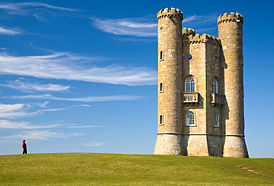
\includegraphics[scale=.7]{figures/seamCarving1.png}}
    \end{subfloatrow}
    \begin{subfloatrow}
        \floatbox[{\capbeside\thisfloatsetup{capbesideposition={right,center},capbesidewidth=5cm}}]{figure}[\FBwidth]
        {\caption{The energy of each pixel.}\label{fig:scEnergy}}
        {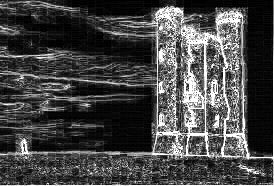
\includegraphics[scale=.7]{figures/seamCarving2.png}}
    \end{subfloatrow}
    \begin{subfloatrow}
        \floatbox[{\capbeside\thisfloatsetup{capbesideposition={right,center},capbesidewidth=5cm}}]{figure}[\FBwidth]
        {\caption{Potential seams to delete.}\label{fig:scSeams}}
        {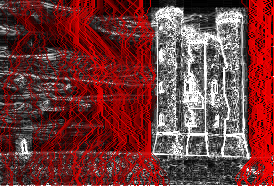
\includegraphics[scale=.7]{figures/seamCarving3.png}}
    \end{subfloatrow}
    \begin{subfloatrow}
        \floatbox[{\capbeside\thisfloatsetup{capbesideposition={right,center},capbesidewidth=11cm}}]{figure}[\FBwidth]
        {\caption{Low energy seams removed.}\label{fig:scRemoved}}
        {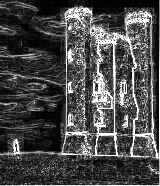
\includegraphics[scale=.7]{figures/seamCarving4.png}}
    \end{subfloatrow}
    \begin{subfloatrow}
        \floatbox[{\capbeside\thisfloatsetup{capbesideposition={right,center},capbesidewidth=9.5cm}}]{figure}[\FBwidth]
        {\caption{Resulting image.}}
        {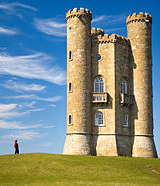
\includegraphics[scale=.7]{figures/seamCarving5.png}}
    \end{subfloatrow}
    \caption[Seam Carving Stages]{Each stage of the seam carving algorithm.}
\end{figure}
